\documentclass[letterpaper]{article}
\usepackage[margin=0.25in]{geometry}
\usepackage{tikz}
\usepackage{fontspec}
\usepackage{xcolor}

% ============================================================================
% COLOR PALETTE (B&W printer friendly - maximum contrast)
% ============================================================================
\definecolor{parkbrown}{RGB}{0, 0, 0}         % Pure black for headers/borders
\definecolor{mutedtext}{RGB}{0, 0, 0}         % Pure black for all text
\definecolor{rulelight}{RGB}{100, 100, 100}   % Medium gray lines

% ============================================================================
% TYPOGRAPHY
% ============================================================================
\setmainfont{EB Garamond}[
  BoldFont = {EB Garamond},
  BoldFeatures = {RawFeature={wght=700}},
  ItalicFont = {EB Garamond Italic},
  BoldItalicFont = {EB Garamond Italic},
  BoldItalicFeatures = {RawFeature={wght=700}}
]

\setsansfont{Josefin Sans}[
  BoldFont = {Josefin Sans},
  BoldFeatures = {RawFeature={wght=700}}
]

\newfontfamily\headerfont{Josefin Sans}[
  RawFeature = {wght=700},
  LetterSpace = 5,
  FakeBold = 1.5
]

\newfontfamily\sectionfont{Josefin Sans}[
  RawFeature = {wght=700},
  FakeBold = 1.5
]

\newfontfamily\promptfont{Caveat}[
  Renderer=HarfBuzz
]

\pagestyle{empty}
\setlength{\parindent}{0pt}

% ============================================================================
% CARD DIMENSIONS (in inches)
% ============================================================================
\def\cardwidth{3.5}
\def\cardheight{5}
\def\gutter{0.25}
\def\headerstrip{0.4}
\def\artboxheight{1.6}
\def\croplen{0.15}

% ============================================================================
% CROP MARKS (for y=-1in coordinate system where y increases downward)
% ============================================================================
\newcommand{\drawcropmarks}[2]{%
  % #1 = x position, #2 = y position (top-left of card)
  % Top-left corner
  \draw[parkbrown, line width=0.3pt] (#1-\croplen,#2) -- (#1,#2);
  \draw[parkbrown, line width=0.3pt] (#1,#2-\croplen) -- (#1,#2);
  % Top-right corner
  \draw[parkbrown, line width=0.3pt] (#1+\cardwidth,#2) -- (#1+\cardwidth+\croplen,#2);
  \draw[parkbrown, line width=0.3pt] (#1+\cardwidth,#2-\croplen) -- (#1+\cardwidth,#2);
  % Bottom-left corner
  \draw[parkbrown, line width=0.3pt] (#1-\croplen,#2+\cardheight) -- (#1,#2+\cardheight);
  \draw[parkbrown, line width=0.3pt] (#1,#2+\cardheight+\croplen) -- (#1,#2+\cardheight);
  % Bottom-right corner
  \draw[parkbrown, line width=0.3pt] (#1+\cardwidth,#2+\cardheight) -- (#1+\cardwidth+\croplen,#2+\cardheight);
  \draw[parkbrown, line width=0.3pt] (#1+\cardwidth,#2+\cardheight+\croplen) -- (#1+\cardwidth,#2+\cardheight);
}

% ============================================================================
% LOCATION CARD COMMAND
% ============================================================================
% \locationcard{x}{y}{name}{def-name}{def-desc}{rec-name}{rec-desc}{prompt}
\newcommand{\locationcard}[8]{%
  \begin{scope}[shift={(#1,#2)}]
    % Crop marks
    \drawcropmarks{0}{0}

    % WPA-style double border
    \draw[line width=2.5pt, parkbrown] (0,0) rectangle (\cardwidth,\cardheight);
    \draw[line width=0.75pt, parkbrown] (0.06,0.06) rectangle (\cardwidth-0.06,\cardheight-0.06);

    % Header strip with location name (at TOP of card)
    \fill[parkbrown] (0.06,0.06) rectangle (\cardwidth-0.06,\headerstrip);
    \node[anchor=center, text=white] at (\cardwidth/2, 0.23) {%
      {\headerfont\fontsize{12}{14}\selectfont #3}%
    };

    % Art placeholder (dashed rectangle below header)
    \draw[parkbrown, dashed, line width=0.75pt]
      (0.15, \headerstrip+0.1) rectangle (\cardwidth-0.15, \headerstrip+0.1+\artboxheight);
    \node[anchor=center, text=rulelight, font=\fontsize{8}{10}\selectfont]
      at (\cardwidth/2, \headerstrip+0.1+\artboxheight/2) {[illustration]};

    % Defense section
    \def\defsectiontop{2.2}
    \draw[parkbrown, line width=0.5pt] (0.1,\defsectiontop) -- (\cardwidth-0.1,\defsectiontop);
    \node[anchor=north west, text=parkbrown] at (0.15,\defsectiontop+0.02) {%
      {\sectionfont\fontsize{7}{8}\selectfont DEFENSE}%
    };
    \node[anchor=north west, text=mutedtext, text width=3.1in] at (0.15,\defsectiontop+0.22) {%
      {\fontsize{9}{11}\selectfont\bfseries #4}\\[-2pt]
      {\fontsize{8}{10}\selectfont #5}%
    };

    % Recovery section
    \def\recsectiontop{3.25}
    \draw[parkbrown, line width=0.5pt] (0.1,\recsectiontop) -- (\cardwidth-0.1,\recsectiontop);
    \node[anchor=north west, text=parkbrown] at (0.15,\recsectiontop+0.02) {%
      {\sectionfont\fontsize{7}{8}\selectfont RECOVERY}%
    };
    \node[anchor=north west, text=mutedtext, text width=3.1in] at (0.15,\recsectiontop+0.22) {%
      {\fontsize{9}{11}\selectfont\bfseries #6}\\[-2pt]
      {\fontsize{8}{10}\selectfont #7}%
    };

    % Prompt section (at bottom)
    \def\promptsectiontop{4.2}
    \draw[parkbrown, line width=0.5pt] (0.1,\promptsectiontop) -- (\cardwidth-0.1,\promptsectiontop);
    \node[anchor=north west, text=mutedtext, text width=3.1in] at (0.15,\promptsectiontop+0.08) {%
      {\promptfont\fontsize{9}{12}\selectfont ``#8''}%
    };
  \end{scope}
}

\begin{document}

% ============================================================================
% PAGE 1: Cards 1-4
% ============================================================================
\noindent
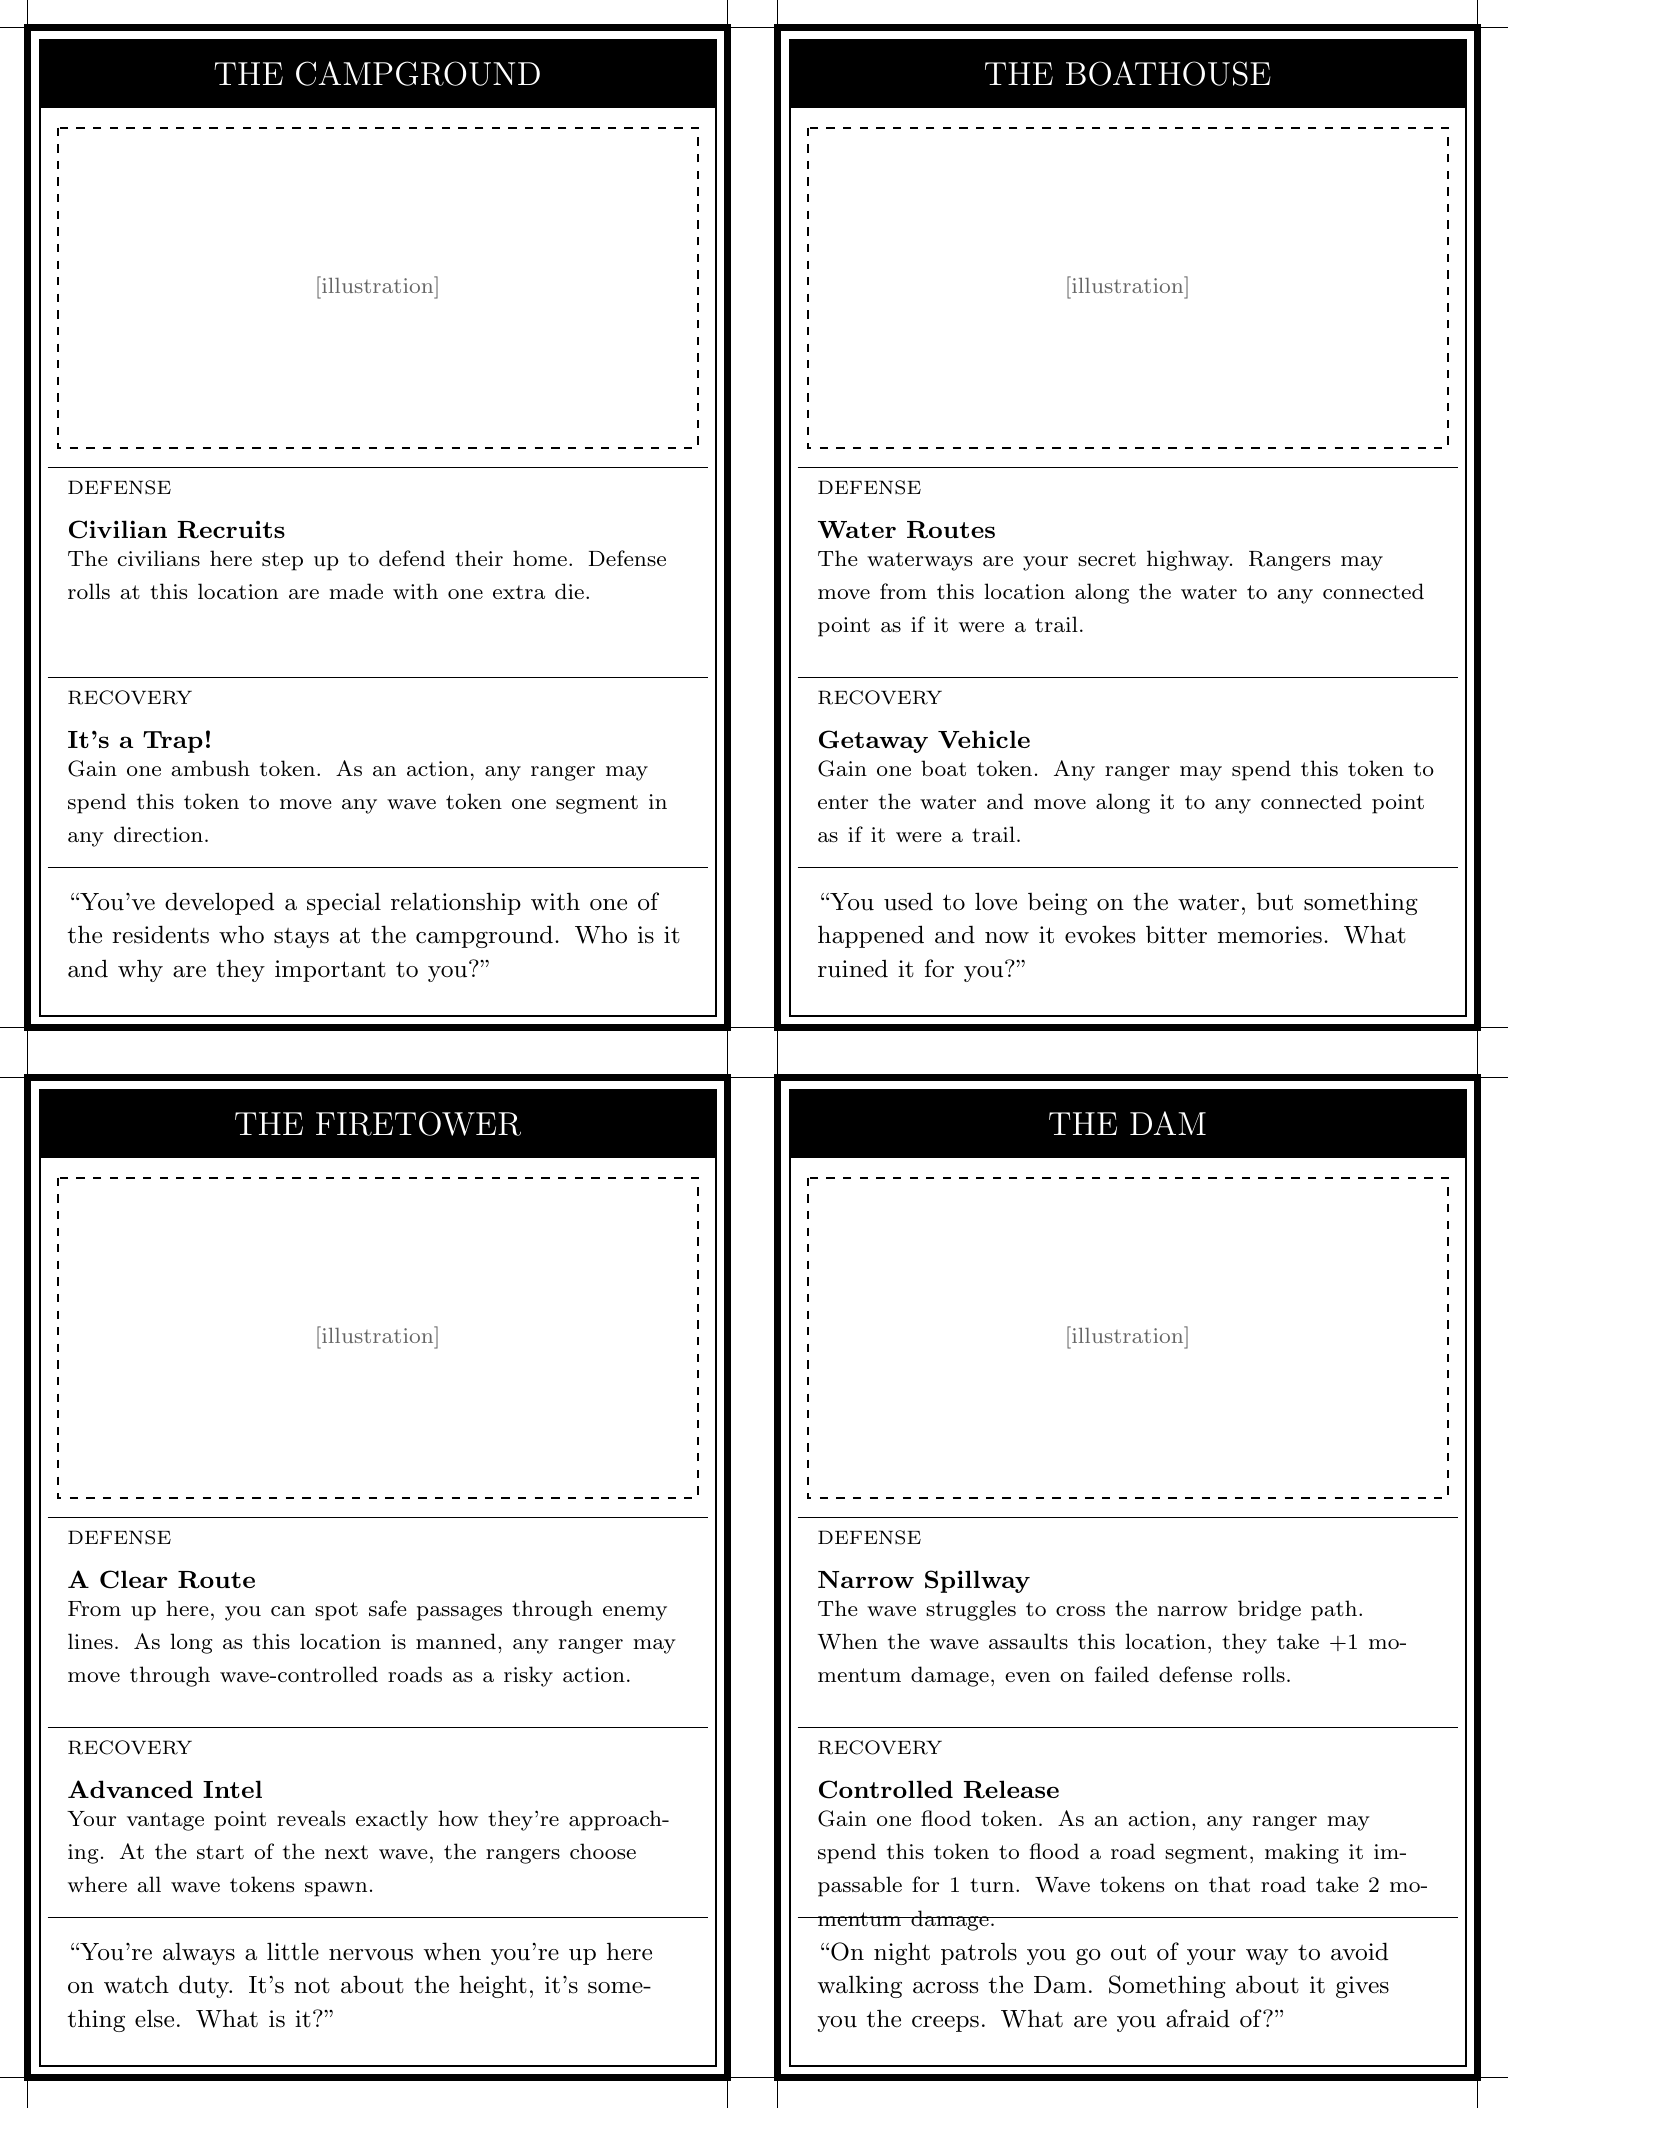
\begin{tikzpicture}[x=1in, y=-1in, every node/.style={text=black}]

  % Set bounding box (with y=-1in, positive y is DOWN, so max y = 10.5 goes to -10.5in)
  \path[use as bounding box] (0,0) -- (8,0) -- (8,10.5) -- (0,10.5) -- cycle;

  % Card positions: 2x2 grid (y=-1in means positive y goes DOWN)
  % Row 1: y=0, Row 2: y=5.25 (card height + gutter)
  % Col 1: x=0, Col 2: x=3.75 (card width + gutter)

  % The Campground (top-left)
  \locationcard{0}{0}%
    {THE CAMPGROUND}%
    {Civilian Recruits}%
    {The civilians here step up to defend their home. Defense rolls at this location are made with one extra die.}%
    {It's a Trap!}%
    {Gain one ambush token. As an action, any ranger may spend this token to move any wave token one segment in any direction.}%
    {You've developed a special relationship with one of the residents who stays at the campground. Who is it and why are they important to you?}

  % The Boathouse (top-right)
  \locationcard{3.75}{0}%
    {THE BOATHOUSE}%
    {Water Routes}%
    {The waterways are your secret highway. Rangers may move from this location along the water to any connected point as if it were a trail.}%
    {Getaway Vehicle}%
    {Gain one boat token. Any ranger may spend this token to enter the water and move along it to any connected point as if it were a trail.}%
    {You used to love being on the water, but something happened and now it evokes bitter memories. What ruined it for you?}

  % The Firetower (bottom-left)
  \locationcard{0}{5.25}%
    {THE FIRETOWER}%
    {A Clear Route}%
    {From up here, you can spot safe passages through enemy lines. As long as this location is manned, any ranger may move through wave-controlled roads as a risky action.}%
    {Advanced Intel}%
    {Your vantage point reveals exactly how they're approaching. At the start of the next wave, the rangers choose where all wave tokens spawn.}%
    {You're always a little nervous when you're up here on watch duty. It's not about the height, it's something else. What is it?}

  % The Dam (bottom-right)
  \locationcard{3.75}{5.25}%
    {THE DAM}%
    {Narrow Spillway}%
    {The wave struggles to cross the narrow bridge path. When the wave assaults this location, they take +1 momentum damage, even on failed defense rolls.}%
    {Controlled Release}%
    {Gain one flood token. As an action, any ranger may spend this token to flood a road segment, making it impassable for 1 turn. Wave tokens on that road take 2 momentum damage.}%
    {On night patrols you go out of your way to avoid walking across the Dam. Something about it gives you the creeps. What are you afraid of?}

\end{tikzpicture}

\newpage

% ============================================================================
% PAGE 2: Cards 5-8
% ============================================================================
\noindent
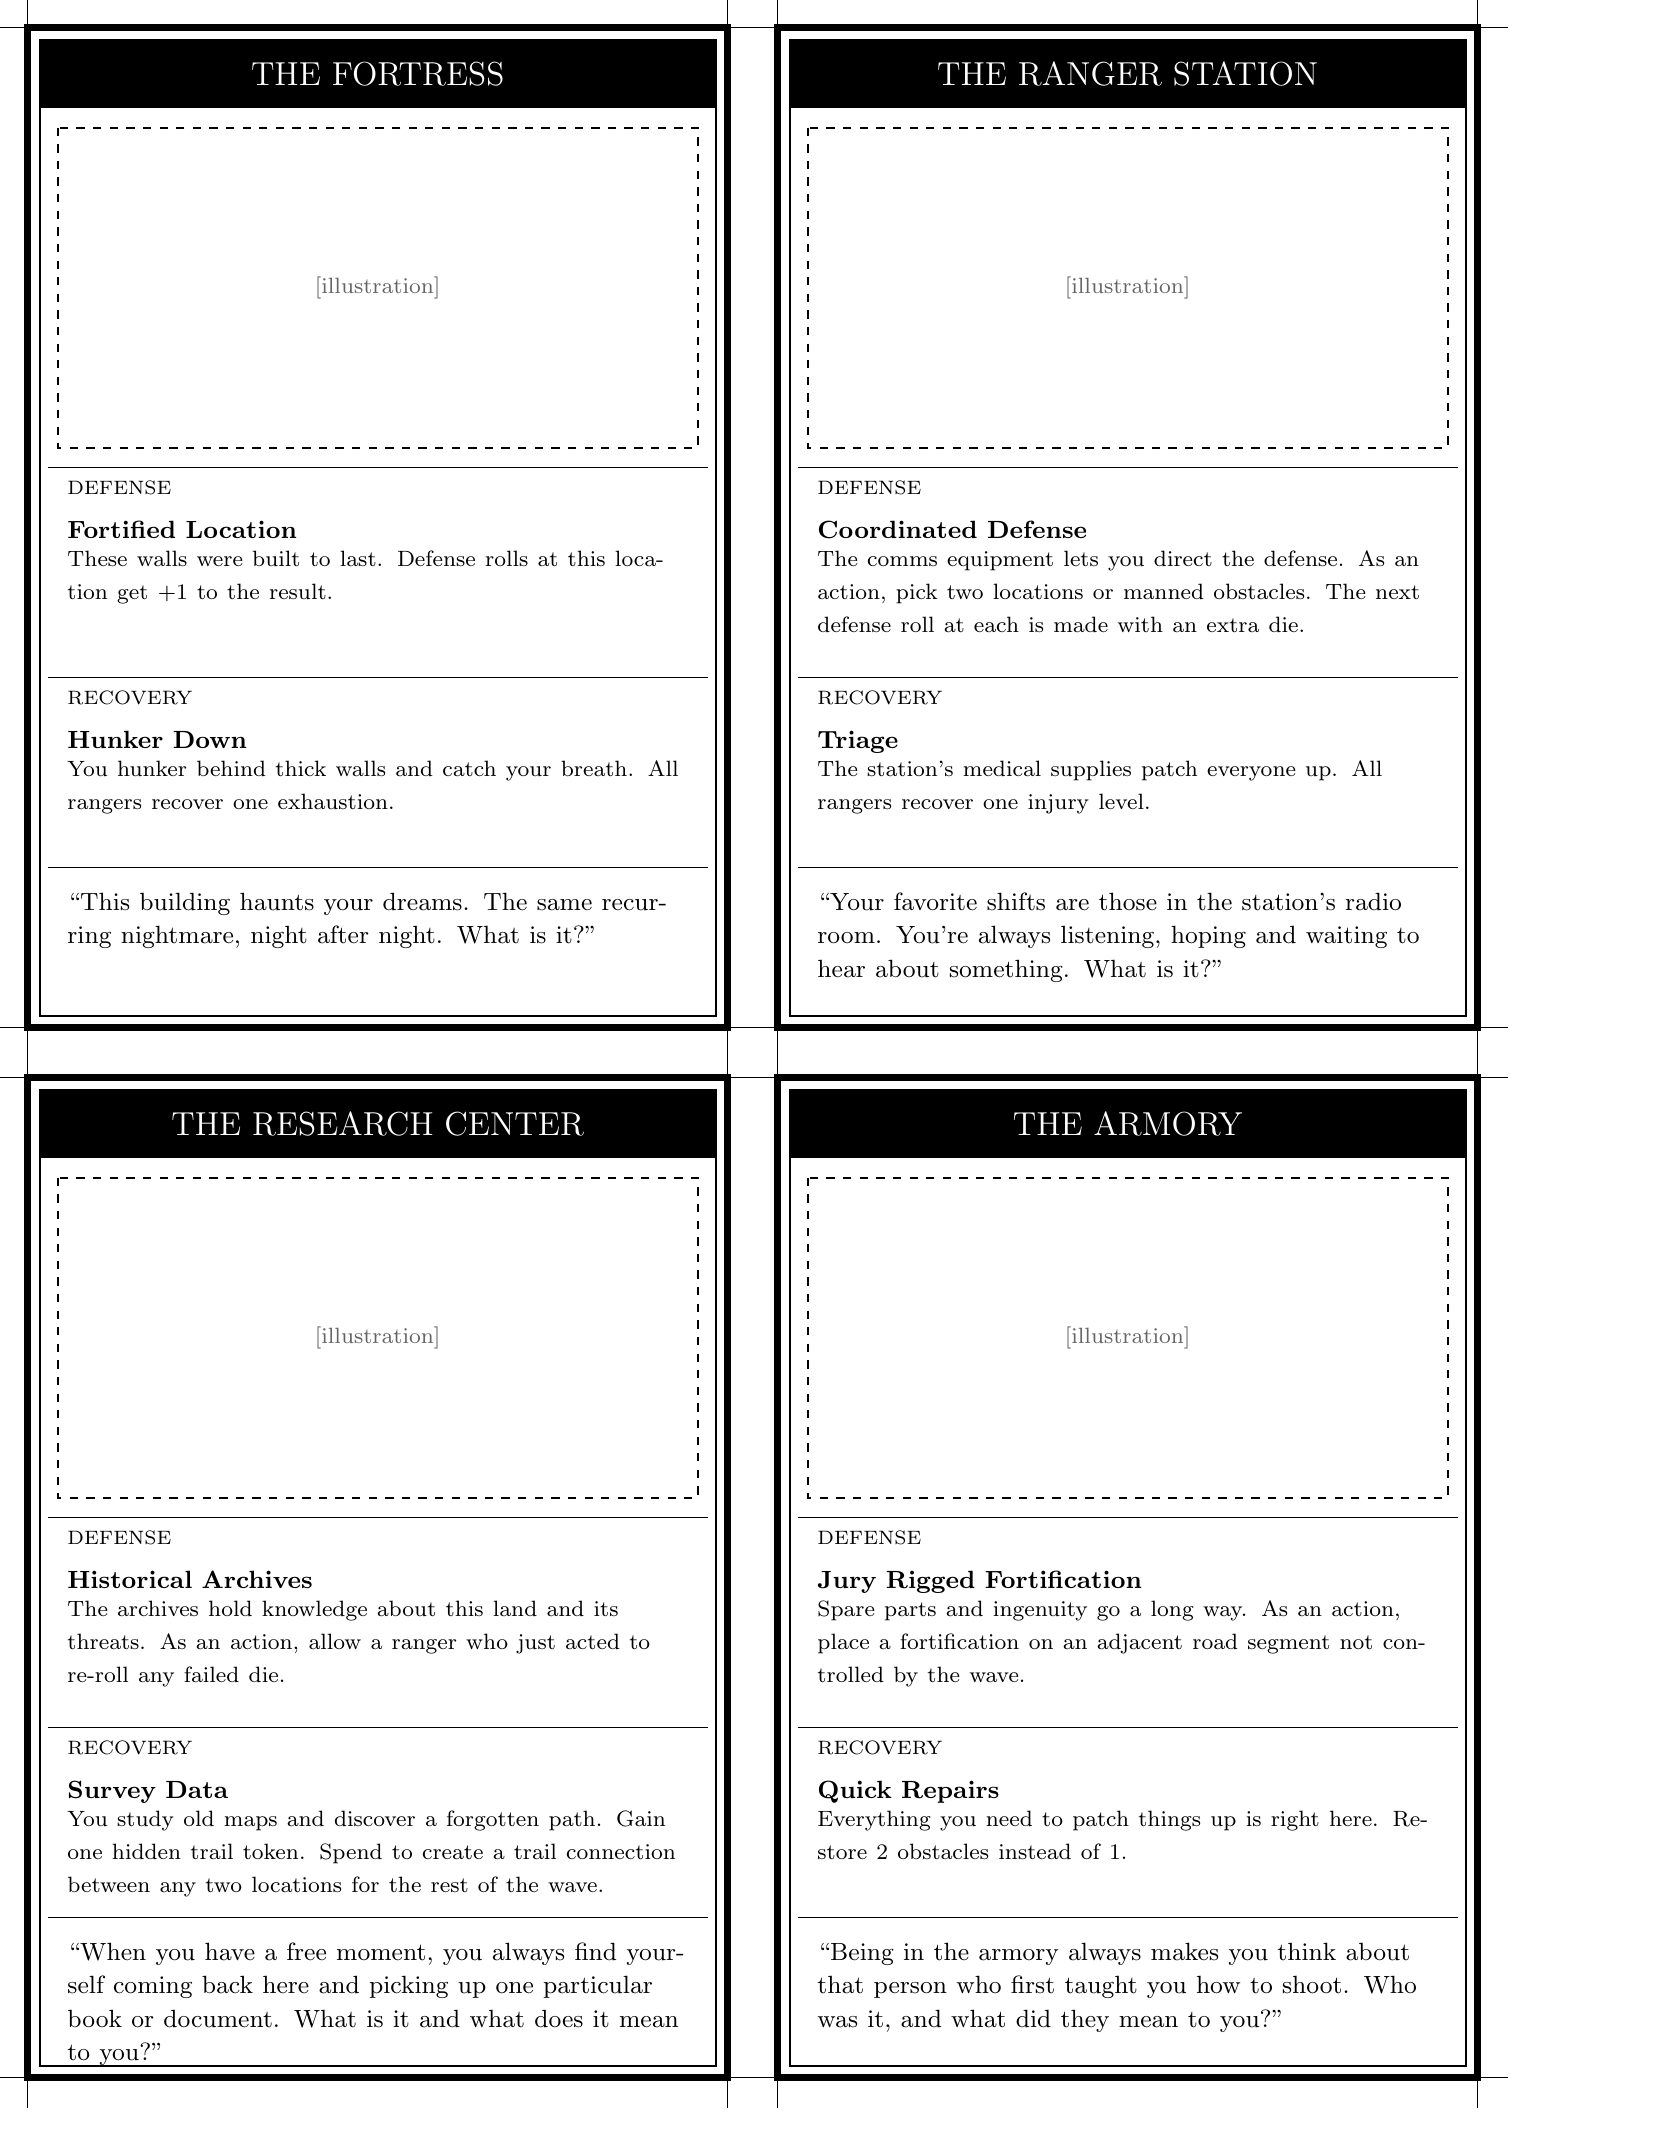
\begin{tikzpicture}[x=1in, y=-1in, every node/.style={text=black}]

  % Set bounding box (with y=-1in, positive y is DOWN, so max y = 10.5 goes to -10.5in)
  \path[use as bounding box] (0,0) -- (8,0) -- (8,10.5) -- (0,10.5) -- cycle;

  % The Fortress (top-left)
  \locationcard{0}{0}%
    {THE FORTRESS}%
    {Fortified Location}%
    {These walls were built to last. Defense rolls at this location get +1 to the result.}%
    {Hunker Down}%
    {You hunker behind thick walls and catch your breath. All rangers recover one exhaustion.}%
    {This building haunts your dreams. The same recurring nightmare, night after night. What is it?}

  % The Ranger Station (top-right)
  \locationcard{3.75}{0}%
    {THE RANGER STATION}%
    {Coordinated Defense}%
    {The comms equipment lets you direct the defense. As an action, pick two locations or manned obstacles. The next defense roll at each is made with an extra die.}%
    {Triage}%
    {The station's medical supplies patch everyone up. All rangers recover one injury level.}%
    {Your favorite shifts are those in the station's radio room. You're always listening, hoping and waiting to hear about something. What is it?}

  % The Research Center (bottom-left)
  \locationcard{0}{5.25}%
    {THE RESEARCH CENTER}%
    {Historical Archives}%
    {The archives hold knowledge about this land and its threats. As an action, allow a ranger who just acted to re-roll any failed die.}%
    {Survey Data}%
    {You study old maps and discover a forgotten path. Gain one hidden trail token. Spend to create a trail connection between any two locations for the rest of the wave.}%
    {When you have a free moment, you always find yourself coming back here and picking up one particular book or document. What is it and what does it mean to you?}

  % The Armory (bottom-right)
  \locationcard{3.75}{5.25}%
    {THE ARMORY}%
    {Jury Rigged Fortification}%
    {Spare parts and ingenuity go a long way. As an action, place a fortification on an adjacent road segment not controlled by the wave.}%
    {Quick Repairs}%
    {Everything you need to patch things up is right here. Restore 2 obstacles instead of 1.}%
    {Being in the armory always makes you think about that person who first taught you how to shoot. Who was it, and what did they mean to you?}

\end{tikzpicture}

\end{document}
